%%Bài toán đề xuất bởi NVPL

\textbf{Rối lượng tử}

Trong Vật Lý lượng tử, phép đo có thể làm thay đổi trạng thái của hệ cần quan sát, dẫn tới sự xuất hiện của tính xác suất trong kết quả thu được. Một hệ quả vô cùng thú vị đến từ tính chất này là khi chúng ta thực hiện đo đạc trên những hạt ở rất xa nhau thì kết quả thu được vẫn có thể liên hệ thống kê với nhau như những sự kiện xảy ra không độc lập, nếu chúng đã {\it rối lượng tử} với nhau. Theo lý thuyết, điều này khả dĩ ngay cả khi vận tốc ánh sáng là không đủ nhanh để truyền tín hiệu giữa chúng. \\
Hiện tượng {\it rối lượng tử} không tồn tại trong Vật Lý cổ điển, rất kỳ lạ và trái ngược trực giác, nên đã tạo ra những bất đồng về diễn giải thế giới lượng tử. Nổi tiếng nhất là cuộc tranh luận giữa những nhà Vật Lý được dẫn dắt bởi Niels Bohr và Albert Einstein, về vấn đề tồn tại hay không một {\it biến số ẩn định xứ} khiến cho các sự kiện lượng tử xảy ra độc lập vẫn có thể biểu hiện liên hệ thống kê với nhau.

Trong bài tập này, chúng ta sẽ đi tìm hiểu cội nguồn của lĩnh vực thông tin lượng tử và cách giải Nobel Vật lý 2022 của 3 nhà vật lý John Clauser, Alain Aspect và Anton Zeilinger chấm dứt cuộc tranh cãi dài một thế kỉ giữa Albert Einstein và Niels Bohr.\\ \\
\textbf{Bài tập này được chia làm hai phần độc lập với nhau và mỗi phần có tổng điểm như một bài.  }

\begin{enumerate}
    \item \textbf{Bất đẳng thức Bell.} \\
    \textit{Rối lượng tử (quantum entanglement)} là một hiện tượng vô cùng "ma quái" của tự nhiên. (Ví dụ trong một số các thí nghiệm lượng tử, hiện tượng rối có thể được tạo ra trong thực tế khi có sự tương tác không tuyến tính giữa các hạt, như quang học phi tuyến, tương tác giữ những nguyên tử Rydberg, ...) Chúng ta hiểu đơn giản rằng sự "ma quái" của rối lượng tử là việc khi ta thực hiện phép đo và biết spin của một trong hai hạt của cặp hạt bị rối lượng tử thì ta \textit{ngay lập tức} biết spin của hạt còn lại bất kể khoảng cách . Như thể hai hạt bị rối đã "nói chuyện" với nhau để tiết lộ thông tin về trạng thái của nhau, điều này ban đầu khiến các nhà vật lý đau đầu vì tưởng rằng rối lượng tử vi phạm thuyết tương đối - không có gì có thể di chuyển nhanh hơn tốc độ truyền thông tin trong chân không - đây chính là \textit{tác dụng ma quái theo khoảng cách (spooky action at a distance)} của cơ học lượng tử. Với hi vọng giải thích cho hiện tượng rối lượng tử mà điều kiện là không vi phạm thuyết tương đối và khớp với quan sát thực nghiệm, Einstein đã đưa ra lý thuyết về việc tồn tại các biến số ẩn chưa biết (tính xác suất của cơ học lượng tử là do chưa biết hết các biến số ẩn này). Lý thuyết biến số ẩn của Einstein đã trở thành cách diễn giải đối lập với quan điểm của Bohr về suy sập hàm sóng do thực hiện phép đo.\\
Năm 1964, John Bell đã đề xuất một phương pháp kiểm chứng cơ học lượng tử và lý thuyết biến ẩn thông qua thí nghiệm giả tưởng về rối lượng tử dựa trên kết quả thực nghiệm đo spin của hai hạt bị rối với nhau luôn luôn cho ra kết quả spin của chúng song song và ngược chiều nhau. Ông giả thuyết tồn tại một biến số ẩn $\lambda$ là thông số liên tục và đơn nhất vào trong hàm sóng. Ông tổng quát phép đo spin của hai hạt bị rối với nhau như sau:\\ \\
"Đo spin $\Vec{\sigma}_1$ của hạt 1 trên phương $\Vec{a}$ và đo spin $\Vec{\sigma}_2$ của hạt 2 trên phương $\Vec{b}$ với $\Vec{a}$ và $\Vec{b}$ là hai vector đơn vị bất kỳ. Spin của hạt 1 "hướng lên" khi song song và cùng chiều với $\Vec{a}$, tức là $\Vec{\sigma}_1 \cdot \Vec{a}=+1$ và "hướng xuống" khi song song và ngược chiều với $\Vec{a}$, tức là $\Vec{\sigma}_1 \cdot \Vec{a}=-1$ . Kết quả phép đo $A(\Vec{a},\lambda)$ của phép đo spin hạt 1 trên $\Vec{a}$ được xác định bởi $\Vec{a}$ và $\lambda$. Tương tự với hạt 2 và kết quả phép đo $B(\Vec{b},\lambda)$. Giả thiết \textbf{kết quả phép đo $A$ hoàn toàn không ảnh hưởng đến kết quả phép đo $B$ và ngược lại}"\\ 

\begin{enumerate}[label=\textbf{\alph*,}]\itemsep0em
    \item Kết quả phép đo $A(\Vec{a},\lambda)$ và phép đo $B(\Vec{b},\lambda)$ có thể nhận những giá trị nào tương ứng với trường hợp nào ?\\
    \item Cách tính giá trị trung bình của kết quả phép đo $\Vec{\sigma}_1$ đo trên $\Vec{a}$ và $\Vec{\sigma}_2$ đo trên $\Vec{b}$ xảy ra đồng thời được định nghĩa như sau:
$$P(\Vec{a},\Vec{b})=\displaystyle\int\limits_{-\infty}^{+\infty}A(\Vec{a},\lambda)B(\Vec{b},\lambda)\rho(\lambda)d\lambda=-\Vec{a}\cdot \Vec{b}.$$
Trong đó $\rho(\lambda)$ là phân bố xác suất của $\lambda$ trong toàn không gian với điều kiện $\rho(\lambda) \geq 0$ và $\displaystyle\int\limits_{-\infty}^{+\infty}\rho(\lambda)d\lambda=1$. \\
Ta giả thiết tồn tại lý thuyết biến ẩn, xét trường hợp đặc biệt khi $\Vec{a} = \Vec{b}$, hai hạt rối lượng tử với nhau luôn đo ra spin song song nhưng ngược chiều với nhau theo thực nghiệm. Với trường hợp đặc biệt này, hãy:
        \begin{enumerate}
            \item Biểu diễn kết quả phép đo $B$ theo $A$.
            \item Tính giá trị trung bình của kết quả phép đo $\Vec{\sigma}_1$ đo trên $\Vec{a}$ và $\Vec{\sigma}_2$ đo trên $\Vec{b}$ khi hai phép đo này xảy ra đồng thời.
            \item Biểu diễn lại giá trị trung bình $P(\Vec{a},\Vec{b})$ chỉ theo $A$ và $\rho(\lambda)$.
        \end{enumerate}
      \item Do ta chọn $\Vec{a}$ và $\Vec{b}$ là hai vector đơn vị bất kỳ nên ta có thể chọn một vector đơn vị $\Vec{c}$ và tính toán phép đo trên $\Vec{a}$ và $\Vec{c}$. Hãy biểu diễn giá trị trung bình $P(\Vec{a},\Vec{c})$ chỉ theo $A$ và $\rho(\lambda)$.
      \item Vì ta đã xây dựng lý thuyết này dựa trên lý thuyết biến ẩn nên ta không chỉ có thể kết luận lý thuyết biến ẩn là đúng mà còn kết luận cơ học lượng tử theo quan điểm của Bohr sai nếu bất kỳ trường hợp nào của $\Vec{a}$, $\Vec{b}$ và $\Vec{c}$ đều thoả mãn điều kiện nào đó giữa $P(\Vec{a},\Vec{b})$, $P(\Vec{a},\Vec{c})$ và $P(\Vec{b},\Vec{c})$. Ngược lại nếu không thì ta có thể kết luận lý thuyết biến ẩn là không tồn tại và cơ học lượng tử theo quan điểm của Bohr là đầy đủ.
      \begin{enumerate}
          \item Tìm điều kiện của hiệu $P(\Vec{a},\Vec{b})-P(\Vec{a},\Vec{c})$ theo $P(\Vec{b},\Vec{c})$.
          \item Thay thử trường hợp $\Vec{a}$ và $\Vec{b}$ tạo với nhau một góc $90^o$ còn $\Vec{c}$ tạo với $\Vec{a}$ và $\Vec{b}$ một góc $45^o$, từ kết quả thu được, theo bạn lý thuyết biến ẩn là đúng hay sai ?
      \end{enumerate}
\end{enumerate}
\item \textbf{Kiểm chứng bất đẳng thức Bell bằng thực nghiệm và giải Nobel 2022.}\\
Sau khi bất đẳng thức Bell ra đời, rất nhiều nhà vật lý cố gắng kiểm chứng tính đúng đắn của bất đẳng thức này bằng thực nghiệm, một trong những thí nghiệm đầu tiên là của John Clauser đề xuất năm 1972, bằng việc đo độ phân cực của cặp photon bị rối lượng tử với nhau. Thí nghiệm của Clauser còn nhiều lỗ hổng nên chưa được chấp nhận rộng rãi mà đến mãi năm 2005, các lỗ hổng mới được lấp hết bởi thí nghiệm của Alain Aspect năm 1982 và của Anton Zeilinger năm 2005. Cả ba thí nghiệm chỉ ra cơ học lượng tử theo quan điểm của Bohr đúng, rối lượng tử không vi phạm thuyết tương đối và buộc tất cả các nhà vật lý phải thừa nhận sự tồn tại của "tác dụng ma quái theo khoảng cách", chấm dứt cuộc tranh cãi một thế kỉ giữa Albert Einstein và Niels Bohr!\\
Trong bài toán này ta sẽ tìm hiểu thí nghiệm của Alain Aspect. Giả sử ta có nguồn sáng S phát ra một cặp photon có tần số khác nhau, di chuyển ngược chiều nhau dọc theo trục $z$. Chúng ta không thể gán cho từng photon một trạng thái xác định, cũng như sự phân cực của từng photon. Photon 1 bay đến đầu đo I, phân cực theo phương $\Vec{a}$ cùng lúc photon 2 bay đến đầu đo II, phân cực theo phương $\Vec{b}$. Khi đến kính phân cực, photon có thể đi qua hoặc không đi qua, được thu bằng kênh $(+)$ và $(-)$ tương ứng \textbf{(Hình 1)}.
\begin{center}
    \begin{figure}[htp]
    \begin{center}
        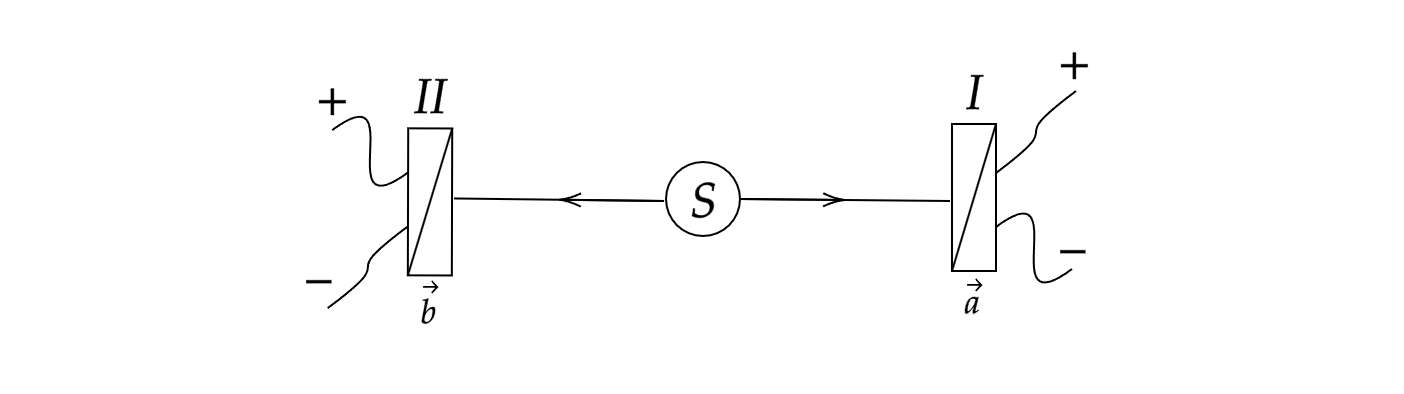
\includegraphics[scale=.25
        ]{Problem_15/image/1.png}
    \end{center}
    \begin{center}
    Hình 1: Thí nghiệm đo phân cực của một cặp photon bị rối
    \end{center}
    \end{figure}
\end{center}
Theo diễn giải cơ học lượng tử của Bohr, xác suất để ngẫu nhiên một photon đi qua $(+)$ một kính phân cực bằng xác suất để nó không đi qua $(-)$: $$P_+(\Vec{a})=P_-(\Vec{a})=\dfrac{1}{2},$$ $$P_+(\Vec{b})=P_-(\Vec{b})=\dfrac{1}{2}.$$
Cũng theo quan điểm này của Bohr, với hệ photon như thí nghiệm của Aspect có xác suất để cả hai photon cùng đi qua $(++)$ hai kính phân cực hoặc cùng không đi qua $(--)$ là bằng nhau và xác suất để một trong hai đi qua kính phân cực I $(+-)$ hoặc II $(-+)$ là bằng nhau: $$P_{++}(\Vec{a},\Vec{b})=P_{--}(\Vec{a},\Vec{b})=\dfrac{1}{2}\cos^2\theta,$$
$$P_{+-}(\Vec{a},\Vec{b})=P_{-+}(\Vec{a},\Vec{b})=\dfrac{1}{2}\sin^2\theta.$$
Trong đó $\theta$ là góc tạo bởi $\Vec{a}$ và $\Vec{b}$.
\begin{enumerate}[label=\textbf{\alph*,}]\itemsep0em
    \item Xét trường hợp đặc biệt khi cả hai kính phân cực có cùng phương phân cực, Xác suất để cả hai photon cùng đi, cùng không đi qua và chỉ một trong hai photon đi qua kính phân cực là bao nhiêu ?
    \item Xét đại lượng $E(\Vec{a},\Vec{b})$ được gọi là \textit{"tương quan giữa hai photon"}. Nếu lý thuyết biến ẩn không tồn tại và diễn giải của Bohr đúng, "tương quan" giữa hai photon được xác định là: $$E(\Vec{a},\Vec{b})=P_{++}(\Vec{a},\Vec{b})+P_{--}(\Vec{a},\Vec{b})-P_{+-}(\Vec{a},\Vec{b})-P_{-+}(\Vec{a},\Vec{b}).$$
Nếu lý thuyết biến ẩn tồn tại và diễn giải của Bohr sai, "tương quan" giữa hai photon được xác định là:
$$E(\Vec{a},\Vec{b})=\displaystyle\int\limits_{-\infty}^{+\infty}A(\Vec{a},\lambda)B(\Vec{b},\lambda)\rho(\lambda)d\lambda.$$ Tính biểu thức "tương quan" giữa hai photon chỉ phụ thuộc vào $\theta$ nếu không tồn tại biến số ẩn.
    \item Bây giờ ta xây dựng tiếp thí nghiệm của Aspect, đó là thêm ở đầu đo I kính phân cực có phương $\Vec{a'}$ và thêm ở đầu đo II kính phân cực có phương $\Vec{b'}$ sao cho phương phân cực của các kính tạo thành các góc như \textbf{(Hình 2)}, lúc này photon đi đến đầu đo I phân cực trên phương $\Vec{a}$ và $\Vec{a'}$, tương tự với đầu đo II là $\Vec{b}$ và $\Vec{b'}$ \textbf{(Hình 2)}.
    \begin{center}
    \begin{figure}[htp]
    \begin{center}
        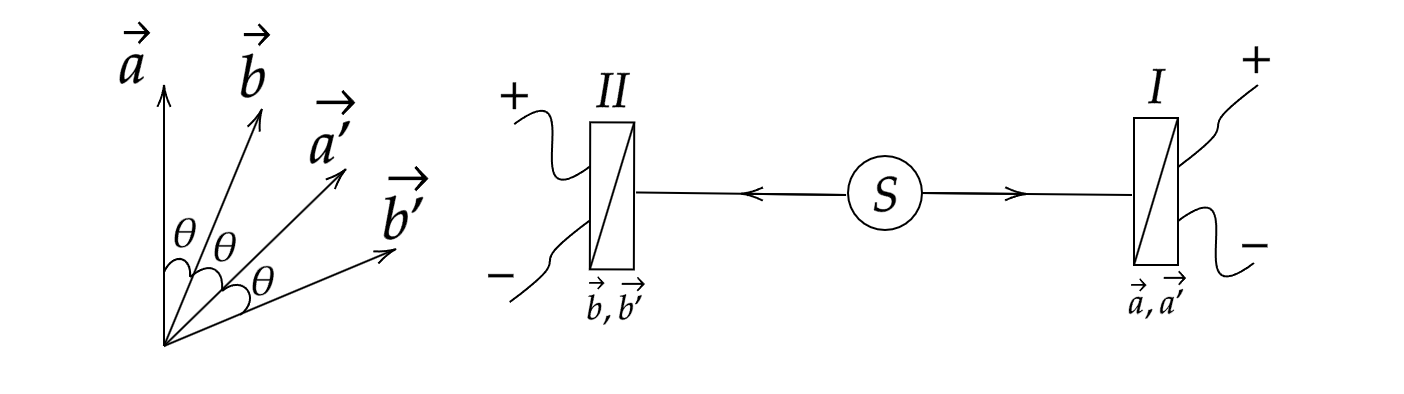
\includegraphics[scale=.25
        ]{Problem_15/image/2.png}
    \end{center}
    \begin{center}
    Hình 2: Thí nghiệm của Alain Aspect
    \end{center}
    \end{figure}
\end{center}
Ta xây dựng biểu thức "tương quan" giữa hai photon dựa trên lý thuyết biến ẩn. Khi tiến hành phép đo hai photon đồng thời với nhau, kết quả phép đo thu được là tổ hợp các trường hợp phân cực có thể xảy ra trên hai đầu đo và bằng tích $AB$. Ta xét đại lượng sau:
$$s(\Vec{a},\Vec{a'},\Vec{b},\Vec{b'},\lambda)=A(\Vec{a},\lambda)B(\Vec{b},\lambda)-A(\Vec{a},\lambda)B(\Vec{b'},\lambda)+A(\Vec{a'},\lambda)B(\Vec{b},\lambda)+A(\Vec{a'},\lambda)B(\Vec{b'},\lambda).$$
Trong đó $A$ và $B$ chỉ có thể nhận các giá trị $-1$ hoặc $+1$.\\
Và giá trị trung bình của đại lượng $s(\Vec{a},\Vec{a'},\Vec{b},\Vec{b'},\lambda)$ được định nghĩa là: $$S(\Vec{a},\Vec{a'},\Vec{b},\Vec{b'})=\displaystyle\int\limits_{-\infty}^{+\infty}s(\Vec{a},\Vec{a'},\Vec{b},\Vec{b'},\lambda)\rho(\lambda)d\lambda.$$
\begin{enumerate}
    \item Đại lượng $s(\Vec{a},\Vec{a'},\Vec{b},\Vec{b'},\lambda)$ chỉ có thể nhận những giá trị nào ?
    \item Giả sử lý thuyết biến ẩn tồn tại và diễn giải cơ học lượng tử của Bohr sai, xác định điều kiện biên của $S(\Vec{a},\Vec{a'},\Vec{b},\Vec{b'})$.
    \item Giả sử lý thuyết biến ẩn không tồn tại và diễn giải cơ học lượng tử của Bohr đúng, xác định điều kiện biên của $S(\Vec{a},\Vec{a'},\Vec{b},\Vec{b'})$.
    \item Đồ thị bên dưới \textbf{(Hình 3)} là kết quả thực nghiệm của Aspect đo đại lượng $S(\Vec{a},\Vec{a'},\Vec{b},\Vec{b'})$ khi thay đổi góc $\theta$. Dựa vào kết quả bạn tìm được ở trên, theo bạn từ kết quả thực nghiệm, lý thuyết biến ẩn đúng hay diễn giải cơ học lượng tử của Bohr đúng? Vậy Einstein hay Bohr đã sai về sự tồn tại của biến số ẩn?
    \begin{center}
    \begin{figure}[htp]
    \begin{center}
        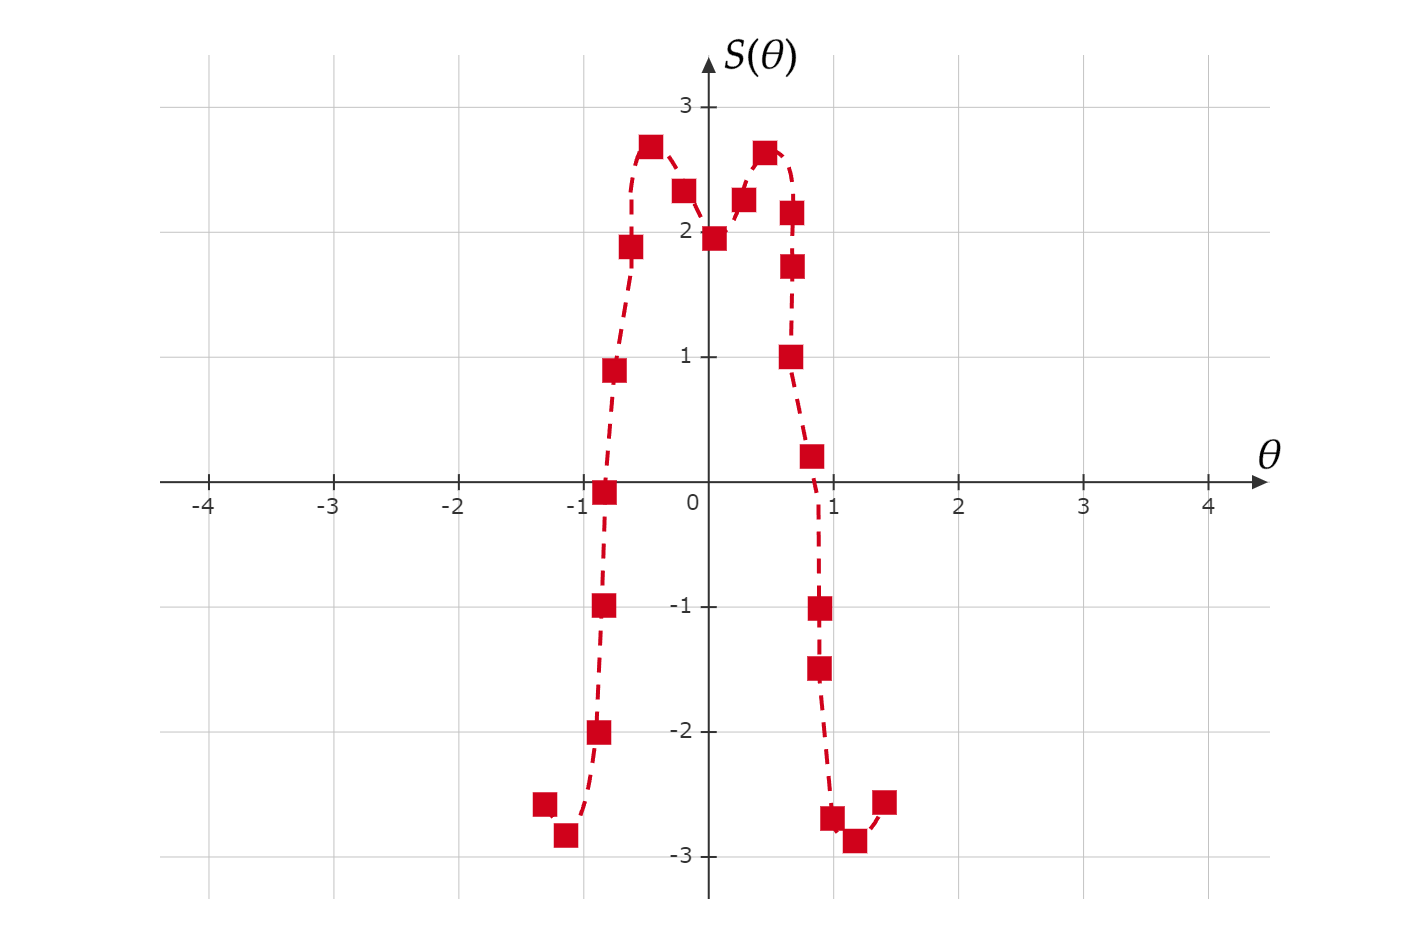
\includegraphics[scale=.22
        ]{Problem_15/image/3.png}
    \end{center}
    \begin{center}
    Hình 3: Kết quả thực nghiệm
    \end{center}
    \end{figure}
\end{center}
\end{enumerate}
\end{enumerate}

\end{enumerate}
\begin{flushright}
    (Biên soạn bởi Nhân viên phòng lab)
\end{flushright}